% Provenance (never printed): cycle 3 / 6e "La planete Terre" (water in the
% ground, groundwater, springs and wells; resource); see
% sources/book1/PROVENANCE.md. Book 1, grade 6, chapter 5.
% Vocabulary guard: "sediment" not before g7.4; the water cycle is recalled
% from the physics book (prose only).
\chapter{الماء تحت الأرض}\label{ch:g6:water-underground}

في يوم صيفي حار، الحقول جافة والجداول ضحلة. ومع ذلك، عند
سفح تل، لا يزال الماء يخرج من الأرض، باردًا صافيًا، كما
كان يخرج طوال الشتاء، ويملأ بركة. ولم تمطر منذ أسابيع. فمن أين يأتي
هذا الماء، وكيف يخرج من \omterm{def:g3:stones-pebbles-sand:rock}{الصخر}؟

\begin{omfigure}
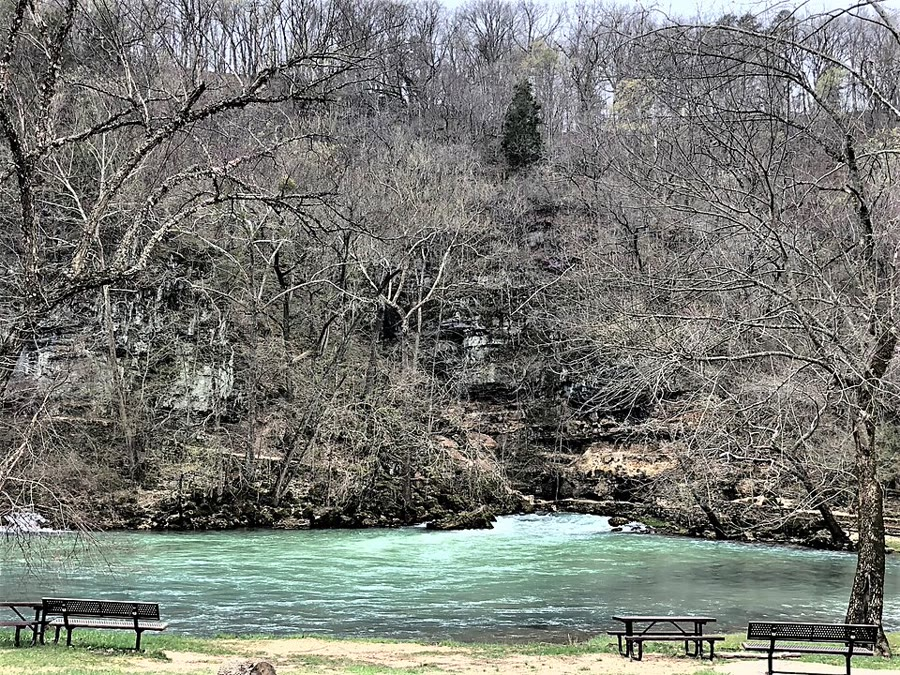
\includegraphics[width=0.72\linewidth]{images/book1/g6-big-spring.jpg}

{\small \omterm{def:g6:water-underground:spring}{ينبوع} يخرج عند سفح جرف صخري ويملأ بركة: بيغ
سبرينغ، ميزوري (الولايات المتحدة). (الصورة: Johnston9494، CC BY-SA 4.0، عبر
ويكيميديا كومنز.)}
% ledger: commons:big-spring
\end{omfigure}

\begin{recall}
يكاد كل الماء على الأرض أن يكون ماءً مالحًا؛ \omterm{def:g2:water-on-earth:salt-fresh}{والماء العذب} جزء صغير منه،
محفوظ في معظمه جليدًا وتحت الأرض
(\cref{ch:g2:water-on-earth}). \omterm{def:g3:stones-pebbles-sand:rock}{والصخور} مثل الحجر الرملي والحجر الجيري
مكوَّنة من حبيبات أو أصداف ملتصقة بعضها ببعض، بينما يتكون الطين والسجّيل من
دقائق ناعمة جدًا (\cref{ch:g6:rocks-and-minerals}). وفي كتاب الفيزياء،
تتبعت الماء في دورته: فهو يتبخر من
البحار، ويتكاثف سحبًا، ثم يعود فيسقط مطرًا أو ثلجًا.
\end{recall}

\section{المطر يتسرب}

حين يسقط \omterm{def:g4:clouds-rain-snow:precipitation}{المطر} على اليابسة، يمكن أن يسلك الماء ثلاثة طرق. فجزء منه
يتبخر عائدًا إلى الهواء. وجزء يجري على السطح، نزولًا مع
المنحدرات، إلى الجداول \omterm{def:g1:landscapes-around-us:water}{والأنهار}: وهذا هو \emph{الجريان السطحي}. والباقي يتسرب
في الأرض.

\begin{definition}[التسرب]\label{def:g6:water-underground:infiltration}
\emph{التسرب}\index{تسرب} هو نفاذ ماء \omterm{def:g4:clouds-rain-snow:precipitation}{المطر}، أو
\omterm{def:g4:clouds-rain-snow:precipitation}{الثلج} الذائب، في الأرض، عبر التربة ونزولًا إلى \omterm{def:g3:stones-pebbles-sand:rock}{الصخور}.
\end{definition}

كمية الماء التي تتسرب تتوقف على الأرض. فعلى منحدر شديد، أو على أرض عارية
أو صلبة، أو على طريق أو موقف سيارات، أو حين تكون التربة مشبعة
بالماء من قبل، يجري معظم الماء على السطح. أما على منحدر لطيف، وتحت العشب
والأشجار، وعلى تربة رملية، فيجد قسم أكبر منه وقتًا ليتسرب.

\begin{omfigure}
\begin{tikzpicture}[x=1cm, y=1cm]
  % rain
  \foreach \x in {0.3,0.9,...,10.5} \draw[blue!55, thick] (\x,3.9) -- (\x-0.15,3.45);
  % ground: field on the left (gentle), road and town on the right
  \fill[brown!30] (0,0) -- (0,2.2) -- (5.2,1.9) -- (5.6,1.85) -- (10.8,1.1) -- (10.8,0) -- cycle;
  \draw[green!50!black, line width=2.5pt] (0,2.2) -- (5.2,1.9);
  \fill[gray!70] (5.6,1.85) -- (10.8,1.1) -- (10.8,0.98) -- (5.6,1.73) -- cycle;
  \foreach \x in {0.4,1.0,...,4.6} \draw[green!45!black, thick] (\x,{2.2-0.058*\x}) -- ++(0.05,0.28) (\x,{2.2-0.058*\x}) -- ++(-0.06,0.24);
  % infiltration arrows in the field
  \foreach \x in {0.8,1.9,3.0,4.1} \draw[->, blue!70!black, very thick] (\x,{2.0-0.058*\x}) -- ++(0,-1.0);
  \node[font=\scriptsize, blue!70!black, align=center, fill=brown!30] at (2.45,0.45) {التسرب: الماء ينفذ في الأرض};
  % run-off on the road
  \draw[->, blue!70!black, very thick] (6.0,2.05) -- (10.3,1.45);
  \node[font=\scriptsize, blue!70!black, align=center] at (8.3,2.3) {الجريان السطحي: الماء يسيل بعيدًا};
  \node[font=\scriptsize, align=center] at (8.3,0.5) {طريق: أرض صلبة\\ يتسرب فيها قليل من الماء};
  \node[font=\scriptsize] at (2.45,2.75) {مرج};
  % evaporation
  \draw[->, gray, thick, decorate, decoration={snake, amplitude=1.2pt, segment length=5pt}] (4.9,2.2) -- (4.9,3.3);
  \node[font=\scriptsize, gray!60!black, anchor=west] at (5.0,3.0) {التبخر};
\end{tikzpicture}

{\small طرق ماء \omterm{def:g4:clouds-rain-snow:precipitation}{المطر} الثلاثة. في المرج يتسرب قسم كبير منه؛
وعلى الطريق يجري معظمه على السطح.}
\end{omfigure}

\section{الصخور المسامية والصخور النفوذة}

انظر إلى حفنة من \omterm{def:g3:stones-pebbles-sand:sand}{الرمل} الجاف من خلال عدسة مكبرة: بين الحبيبات
فراغات صغيرة جدًا. صُبّ عليها الماء فيملأ الماء هذه الفراغات.
وكثير من \omterm{def:g3:stones-pebbles-sand:rock}{الصخور} كذلك: فهي مليئة بثقوب صغيرة بين حبيباتها،
أو بشقوق رفيعة.

\begin{definition}[المسامية]\label{def:g6:water-underground:porosity}
\emph{مسام}\index{مسام} \omterm{def:g3:stones-pebbles-sand:rock}{الصخر} هي الفراغات الموجودة بين حبيباته
وفي شقوقه. \omterm{def:g3:stones-pebbles-sand:rock}{والصخر} الذي فيه مسام \omterm{def:g3:stones-pebbles-sand:rock}{صخر} \emph{مسامي}\index{مسامي}. و\emph{المسامية}\index{مسامية}
هي الجزء من حجمه الذي تشغله المسام،
مكتوبًا نسبةً مئوية.
\end{definition}

\begin{definition}[النفاذية]\label{def:g6:water-underground:permeability}
يكون \omterm{def:g3:stones-pebbles-sand:rock}{الصخر} \emph{نفوذًا}\index{نفوذ} حين يستطيع الماء أن يجري عبره،
لأن مسامه واسعة بما يكفي ومتصل بعضها ببعض. ويكون
\emph{كتيمًا}\index{كتيم} حين لا يستطيع الماء أن يجري عبره.
و\emph{النفاذية}\index{نفاذية} هي مدى سهولة جريان الماء عبر
\omterm{def:g3:stones-pebbles-sand:rock}{الصخر}.
\end{definition}

الفكرتان ليستا الشيء نفسه. فالطين \omterm{def:g6:water-underground:porosity}{مسامي} جدًا: نصف حجمه
\omterm{def:g6:water-underground:porosity}{مسام}. لكن مسامه دقيقة إلى حد أن الماء يبقى عالقًا
فيها: فالطين \emph{\omterm{def:g6:water-underground:permeability}{كتيم}}. \omterm{def:g3:stones-pebbles-sand:sand}{والرمل} مسامه أقل من \omterm{def:g6:water-underground:porosity}{مسام} الطين، لكنها
واسعة ومتصلة: \omterm{def:g3:stones-pebbles-sand:sand}{فالرمل} \emph{\omterm{def:g6:water-underground:permeability}{نفوذ}}. والغرانيت الخالي من الشقوق
يكاد لا يحوي أي \omterm{def:g6:water-underground:porosity}{مسام}.
% ledger: heath:porosity

\begin{omfigure}
\begin{tikzpicture}
  % sand
  \begin{scope}
    \fill[blue!12] (0,0) rectangle (4.4,3.2);
    \foreach \x/\y/\r in {0.45/0.45/0.42, 1.35/0.4/0.4, 2.3/0.5/0.45, 3.3/0.42/0.4, 4.1/0.5/0.35,
                         0.85/1.25/0.41, 1.85/1.3/0.44, 2.85/1.3/0.4, 3.85/1.3/0.42,
                         0.4/2.1/0.38, 1.35/2.15/0.43, 2.35/2.15/0.4, 3.3/2.12/0.42, 4.15/2.1/0.3,
                         0.85/2.88/0.3, 1.85/2.92/0.3, 2.85/2.9/0.3, 3.8/2.9/0.32}
      \fill[yellow!55!brown!60, draw=brown!60!black] (\x,\y) circle (\r);
    \draw (0,0) rectangle (4.4,3.2);
    \draw[->, blue!70!black, very thick, rounded corners=3pt] (1.35,3.4) -- (1.35,2.62) -- (0.88,2.3) -- (0.88,1.95) -- (1.33,1.72) -- (1.33,0.92) -- (0.91,0.75) -- (0.91,-0.3);
    \node[font=\small, align=center] at (2.2,-0.75) {رمل: مسام واسعة متصلة\\ \emph{مسامي ونفوذ}};
  \end{scope}
  % clay
  \begin{scope}[xshift=6.0cm]
    \fill[blue!12] (0,0) rectangle (4.4,3.2);
    \foreach \y in {0.1,0.3,...,3.0}
      \foreach \x in {0.05,0.85,...,3.7}
        \fill[gray!55, draw=gray!30!black, line width=0.2pt, rotate around={{3*sin(57*\x+91*\y)}:(\x+0.36,\y+0.06)}]
          ({\x+0.05*sin(200*\y)},\y) rectangle ++(0.72,0.13);
    \draw (0,0) rectangle (4.4,3.2);
    \draw[->, blue!70!black, very thick] (2.2,3.75) -- (2.2,3.3);
    \node[font=\scriptsize, blue!70!black] at (3.3,3.55) {الماء يتوقف};
    \node[font=\small, align=center] at (2.2,-0.75) {طين: مسام دقيقة بين رقائق\\ \emph{مسامي لكنه كتيم}};
  \end{scope}
\end{tikzpicture}

{\small \omterm{def:g6:water-underground:porosity}{المسام} (بالأزرق) بين حبيبات \omterm{def:g3:stones-pebbles-sand:sand}{رمل} وبين
رقائق طين، مكبَّرة كثيرًا. يجد الماء طريقه عبر \omterm{def:g3:stones-pebbles-sand:sand}{الرمل}؛ أما في
الطين، فيبقى عالقًا.}
\end{omfigure}

يعطي الجدول \omterm{def:g6:water-underground:porosity}{مسامية} بعض المواد، ونسبة الماء
الذي يُصرَّف منها من تلقاء نفسه حين تكون مملوءة بالماء. والباقي
يبقى عالقًا بالحبيبات.

\begin{center}\small
\begin{tabular}{|l|c|c|}
\hline
\textbf{المادة} & \textbf{\omterm{def:g6:water-underground:porosity}{المسامية} (\%)} & \textbf{الماء الذي يُصرَّف (\%)} \\
\hline
تربة & 55 & 40 \\
طين & 50 & 2 \\
\omterm{def:g3:stones-pebbles-sand:sand}{رمل} & 25 & 22 \\
\omterm{def:g3:stones-pebbles-sand:pebble}{حصباء} & 20 & 19 \\
حجر جيري & 20 & 18 \\
حجر رملي & 11 & 6 \\
غرانيت & 0.1 & 0.09 \\
\hline
\end{tabular}
\end{center}
% ledger: heath:porosity

\begin{method}[كم ماءً يحمل الصخر؟]\label{met:g6:water-underground:volume}
\begin{enumerate}
  \item أوجد حجم \omterm{def:g3:stones-pebbles-sand:rock}{الصخر} (لكتلة: الطول $\times$ العرض
        $\times$ \omterm{def:g4:world-physical-map:altitude}{الارتفاع}).
  \item اضرب في \omterm{def:g6:water-underground:porosity}{المسامية} واقسم على 100: فتحصل على حجم
        \omterm{def:g6:water-underground:porosity}{المسام}، أي الماء الذي يحمله \omterm{def:g3:stones-pebbles-sand:rock}{الصخر} حين يكون مملوءًا.
  \item وللماء الذي يُصرَّف، استعمل النسبة المئوية الثانية بالطريقة
        نفسها. (المتر المكعب الواحد 1000~لتر.)
\end{enumerate}
\end{method}

\begin{example}[متر مكعب من الرمل]\label{ex:g6:water-underground:sand}
المتر المكعب الواحد من \omterm{def:g3:stones-pebbles-sand:sand}{الرمل}، المملوء بالماء، يحمل في مسامه $1000 \times 25 \div 100 =
250$~لترًا من الماء. ومن هذه الكمية، يُصرَّف $1000 \times 22 \div 100 = 220$
لترًا من تلقاء نفسه؛ و30~لترًا تبقى عالقة بالحبيبات. والمتر
المكعب الواحد من الطين يحمل ضعف هذه الكمية من الماء، 500~لتر، لكن لا يُصرَّف منه إلا
20~لترًا.
% ledger: heath:porosity
\end{example}

\begin{inthelab}[رمل أم طين؟ (في القسم، مع المعلم)]
أصيصا زهور في قاع كل منهما ثقب، يقفان فوق كأسين. أحدهما
مملوء \omterm{def:g3:stones-pebbles-sand:sand}{برمل} جاف، والآخر بتربة طينية جافة مكبوسة. ويصب المعلم
الكأس نفسها من الماء في كل منهما، في الوقت نفسه. فعبر
\omterm{def:g3:stones-pebbles-sand:sand}{الرمل}، سرعان ما يقطر الماء في الكأس التي تحته. أما على الطين، فيبقى الماء
في الأعلى بركةً صغيرة ولا تنفذ منه إلا قطرات قليلة، ببطء: \omterm{def:g3:stones-pebbles-sand:sand}{فالرمل}
\omterm{def:g6:water-underground:permeability}{نفوذ}، والطين ليس كذلك.
\end{inthelab}

\section{المياه الجوفية ومنسوبها}

احفر حفرة في \omterm{def:g3:stones-pebbles-sand:sand}{رمل} شاطئ، على بعد خطوات من \omterm{def:g2:water-on-earth:ocean}{البحر}: بعد قليل،
يظهر الماء في قاع الحفرة. لقد وصلت إلى المكان الذي تكون فيه
كل \omterm{def:g6:water-underground:porosity}{مسام} \omterm{def:g3:stones-pebbles-sand:sand}{الرمل} مملوءة بالماء.
% ledger: wss:aquifer

\begin{definition}[المياه الجوفية]\label{def:g6:water-underground:groundwater}
\emph{المياه الجوفية}\index{مياه جوفية} هي الماء الموجود تحت الأرض، الذي
يملأ \omterm{def:g6:water-underground:porosity}{مسام} التربة \omterm{def:g3:stones-pebbles-sand:rock}{والصخور} وشقوقها.
\end{definition}

\begin{definition}[منسوب المياه الجوفية]\label{def:g6:water-underground:water-table}
تحت عمق معيّن، تكون كل \omterm{def:g6:water-underground:porosity}{مسام} \omterm{def:g3:stones-pebbles-sand:rock}{الصخر} مملوءة بالماء.
و\emph{منسوب المياه الجوفية}\index{منسوب المياه الجوفية} هو أعلى هذه المنطقة المملوءة بالماء.
فوقه، تحوي \omterm{def:g6:water-underground:porosity}{المسام} هواءً وقليلًا من الماء؛ وتحته، تكون مملوءة
بالماء.
% ledger: wss:aquifer
\end{definition}

\omterm{def:g6:water-underground:water-table}{منسوب المياه الجوفية} ليس مستويًا. فهو يتبع شكل الأرض، لكن بلطف
أكبر: أعلى تحت \omterm{def:g1:landscapes-around-us:landform}{التلال}، وأخفض تحت \omterm{def:g1:landscapes-around-us:landform}{الأودية}. وهو يرتفع أيضًا
وينخفض مع الفصول. فبعد موسم الأمطار، يرفعه \omterm{def:g4:clouds-rain-snow:precipitation}{المطر} الذي
\omterm{def:g6:water-underground:infiltration}{تسرب}؛ وبعد موسم \omterm{def:g5:natural-hazards:drought}{جفاف} طويل، يجري الماء ببطء نحو
\omterm{def:g6:water-underground:spring}{الينابيع} \omterm{def:g1:landscapes-around-us:water}{والأنهار}، فينخفض \omterm{def:g6:water-underground:water-table}{منسوب المياه الجوفية}.

\omterm{def:g6:water-underground:groundwater}{المياه الجوفية} مخزون عظيم من \omterm{def:g2:water-on-earth:salt-fresh}{الماء العذب}. فمن كل \omterm{def:g2:water-on-earth:salt-fresh}{الماء العذب} على
الأرض، نحو 69~\% جليد وثلوج دائمة، ونحو 30~\% \omterm{def:g6:water-underground:groundwater}{مياه
جوفية}؛ أما \omterm{def:g2:water-on-earth:salt-fresh}{الماء العذب} في كل \omterm{def:g1:landscapes-around-us:water}{البحيرات} فلا يزيد على نحو ربع
واحد في المئة. \omterm{def:g6:water-underground:groundwater}{فالمياه الجوفية} أوفر من \omterm{def:g2:water-on-earth:salt-fresh}{الماء العذب} في \omterm{def:g1:landscapes-around-us:water}{البحيرات} بأكثر من مئة
مرة.
% ledger: wss:fresh-shares

\begin{omfigure}
\begin{tikzpicture}
  \begin{axis}[xbar, width=0.8\linewidth, height=3.9cm, bar width=8pt,
      xmin=0, xmax=85, ymin=-0.6, ymax=4.6, y dir=reverse,
      ytick={0,...,4}, yticklabels={جليد وثلوج دائمة, مياه جوفية, جليد التربة والتربة الصقيعية, بحيرات, كل ما عدا ذلك},
      xlabel={\foreignlanguage{arabic}{النسبة المئوية من كل الماء العذب على الأرض}},
      axis x line=bottom, axis y line=left, axis line style={-},
      tick label style={font=\scriptsize}, label style={font=\small},
      nodes near coords, nodes near coords style={font=\scriptsize, anchor=west},
      point meta=explicit symbolic, enlarge y limits=false, clip=false]
    \addplot[fill=blue!35, draw=blue!60!black] table[x=pct, y=idx, meta=pct] {figdata/out/grade-6-water_table-fresh.dat};
  \end{axis}
\end{tikzpicture}

{\small أين يوجد \omterm{def:g2:water-on-earth:salt-fresh}{الماء العذب} على الأرض. أعمدة \omterm{def:g1:landscapes-around-us:water}{البحيرات}
وكل ما عدا ذلك (\omterm{def:g1:landscapes-around-us:water}{الأنهار}، والهواء، والتربة، والمستنقعات، والكائنات الحية) أقصر
من أن تُرى.}
% ledger: wss:fresh-shares (figdata/grade-6/water_table.py, part fresh)
\end{omfigure}

\section{الينابيع والآبار}

\begin{definition}[الينبوع والبئر]\label{def:g6:water-underground:spring}
\emph{الينبوع}\index{ينبوع} مكان تخرج فيه \omterm{def:g6:water-underground:groundwater}{المياه الجوفية} من
الأرض من تلقاء نفسها، حيث يلتقي \omterm{def:g6:water-underground:water-table}{منسوب المياه الجوفية} بالسطح.
و\emph{البئر}\index{بئر} حفرة تُحفر أو تُثقب إلى ما تحت \omterm{def:g6:water-underground:water-table}{منسوب المياه
الجوفية}، فتملأ \omterm{def:g6:water-underground:groundwater}{المياه الجوفية} قاعها ويمكن رفعها إلى الخارج.
\end{definition}

يقطع المقطع أدناه \omterm{def:g1:landscapes-around-us:landform}{واديًا} من \omterm{def:g1:landscapes-around-us:landform}{وديان} تلال فاردن، منطقة
تماريننا. \omterm{def:g1:landscapes-around-us:landform}{والتلال} مكوَّنة من الطباشير، وهو حجر جيري أبيض طري \omterm{def:g6:water-underground:porosity}{مسامي} \omterm{def:g6:water-underground:permeability}{ونفوذ}.
وتحت الطباشير طبقة من السجّيل، وهو \omterm{def:g6:water-underground:permeability}{كتيم}.
فيتسرب \omterm{def:g4:clouds-rain-snow:precipitation}{المطر} في الطباشير، ويملأ مسامه، ثم يتوقف عند السجّيل.

\begin{omfigure}
\begin{tikzpicture}
\begin{axis}[omsection, width=0.95\linewidth, height=7.2cm,
    xmin=0, xmax=2.8, ymin=0, ymax=560,
    xlabel={\foreignlanguage{arabic}{المسافة من الطرف الجنوبي للمقطع \babelsublr{(km)}}},
    ylabel={\foreignlanguage{arabic}{الارتفاع فوق مستوى سطح البحر \babelsublr{(m)}}},
    tick label style={font=\scriptsize}, label style={font=\small},
    clip mode=individual]
  \addplot[om lith={icsJurassic!40}{om limestone}, draw=black, line width=0.3pt, even odd rule] table {figdata/out/grade-6-water_table-unit-limestone.dat};
  \addplot[om lith={icsJurassic!15}{om shale}, draw=black, line width=0.3pt, even odd rule] table {figdata/out/grade-6-water_table-unit-shale.dat};
  \addplot[om lith={icsCretaceous!35}{om limestone}, draw=black, line width=0.3pt, even odd rule] table {figdata/out/grade-6-water_table-unit-chalk.dat};
  \addplot[lith alluvium, draw=black, line width=0.3pt, even odd rule] table {figdata/out/grade-6-water_table-unit-alluvium.dat};
  \addplot[black, thick] table {figdata/out/grade-6-water_table-ground.dat};
  \addplot[blue!75!black, very thick] table {figdata/out/grade-6-water_table-wet.dat};
  \addplot[blue!75!black, very thick, dashed] table {figdata/out/grade-6-water_table-dry.dat};
  % wells
  \addplot[fill=white, draw=black, line width=0.4pt] table {figdata/out/grade-6-water_table-well-rects.dat};
  \node[font=\scriptsize\bfseries, anchor=south east, fill=white, fill opacity=0.8, text opacity=1, inner sep=1pt] at (axis cs:1.45,401.3) {\foreignlanguage{arabic}{البئر~A}};
  \node[font=\scriptsize\bfseries, anchor=south east, fill=white, fill opacity=0.8, text opacity=1, inner sep=1pt] at (axis cs:1.7,470.3) {\foreignlanguage{arabic}{البئر~B}};
  % river and spring
  \addplot[only marks, mark=*, mark size=2.2pt, blue!75!black] table[x=s_km, y=z_m] {figdata/out/grade-6-water_table-points.dat};
  \node[font=\scriptsize, blue!70!black, anchor=south east] at (axis cs:0.215,140) {نهر};
  \node[font=\scriptsize, blue!70!black, anchor=east] at (axis cs:0.83,218) {ينبوع};
  \node[font=\scriptsize] at (axis cs:2.2,470) {الطباشير، وهو نفوذ};
  \node[font=\scriptsize, fill=white, fill opacity=0.8, text opacity=1] at (axis cs:2.2,95) {السجّيل، وهو كتيم};
  \node[font=\scriptsize, fill=white, fill opacity=0.8, text opacity=1] at (axis cs:0.95,25) {حجر جيري};
  \node[font=\scriptsize, blue!70!black, fill=white, fill opacity=0.8, text opacity=1, align=center] at (axis cs:2.15,250) {منسوب المياه الجوفية\\ بعد موسم الأمطار: خط متصل\\ بعد موسم الجفاف: خط متقطع};
\end{axis}
\end{tikzpicture}

{\small مقطع من الشمال إلى الجنوب عبر تلال فاردن، من \omterm{def:g1:landscapes-around-us:water}{النهر} صعودًا على
السفح الشمالي (الارتفاعات مضخَّمة نحو مرتين). والماء المخزون في
الطباشير يتوقف عند السجّيل ويخرج ينبوعًا حيث تلتقي قاعدة
الطباشير بالمنحدر. \omterm{def:g6:water-underground:spring}{والبئر}~A تصل إلى الماء دائمًا؛ أما \omterm{def:g6:water-underground:spring}{البئر}~B فلا تصل
إليه إلا بعد موسم الأمطار.}
% (figdata/grade-6/water_table.py; region model figdata/shared/region.py)
\end{omfigure}

يجري \omterm{def:g6:water-underground:spring}{الينبوع} حيث تلتقي قاعدة الطباشير بالسفح: فالماء
لا يستطيع أن ينزل عبر السجّيل، فيجري على سطح السجّيل
ويخرج على المنحدر. وما دام في الطباشير ماء فوق
السجّيل، يظل \omterm{def:g6:water-underground:spring}{الينبوع} جاريًا، حتى في صيف جاف: وهذا هو
الجواب عن السؤال الذي طُرح في أول الفصل.

انظر إلى البئرين. عمق \omterm{def:g6:water-underground:spring}{البئر}~A 100~متر؛ وقاعها تحت \omterm{def:g6:water-underground:water-table}{منسوب المياه
الجوفية} في كل الفصول، لذلك تعطي الماء دائمًا. \omterm{def:g6:water-underground:spring}{والبئر}~B أعمق منها،
105~أمتار، لكنها حُفرت في موضع أعلى من التل: فقاعها تحت \omterm{def:g6:water-underground:water-table}{منسوب المياه
الجوفية} بعد موسم الأمطار وفوقه بعد موسم \omterm{def:g5:natural-hazards:drought}{الجفاف}. وفي الصيف،
تجف \omterm{def:g6:water-underground:spring}{البئر}~B. فالمهم ليس عمق \omterm{def:g6:water-underground:spring}{البئر}، بل المسافة التي ينزلها
قاعها تحت أدنى منسوب \omterm{def:g6:water-underground:groundwater}{للمياه الجوفية}.
% (figdata/grade-6/water_table.py, part wells)

\begin{omfigure}
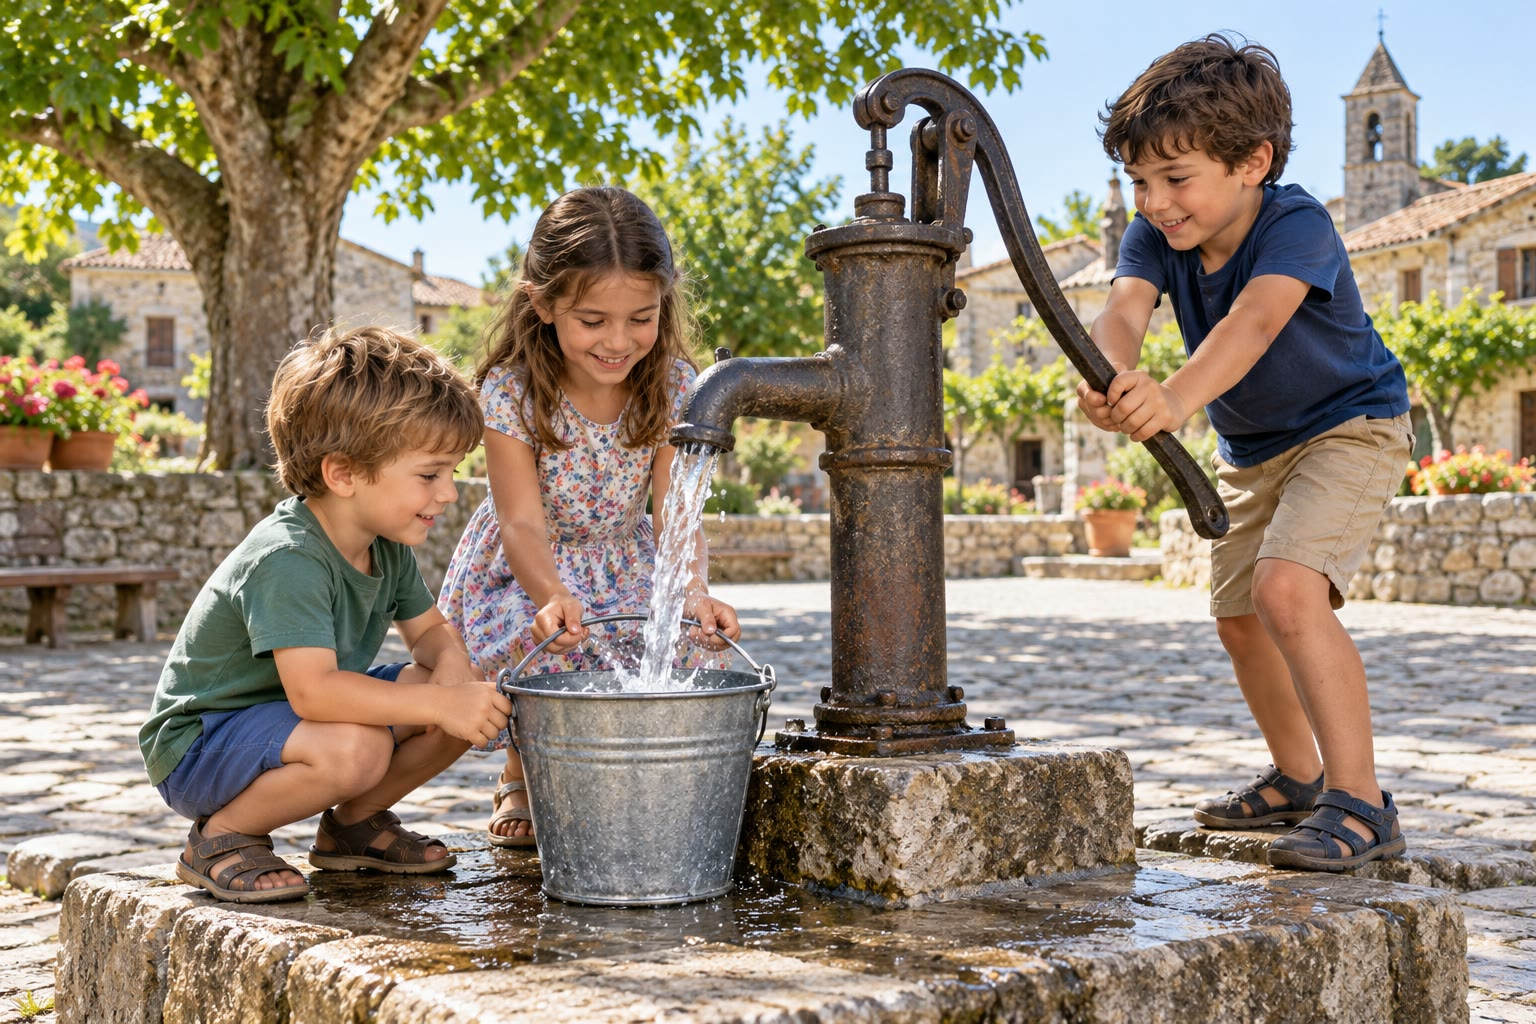
\includegraphics[width=0.6\linewidth]{images/book1/ai/g6-hand-pump.jpg}

{\small أطفال يملؤون دلوًا من المضخة اليدوية \omterm{def:g6:water-underground:spring}{لبئر} القرية. (رسم
بالذكاء الاصطناعي.)}
\end{omfigure}

\begin{remark}[قد تجف البئر]\label{rem:g6:water-underground:pumping}
ضخ الماء من \omterm{def:g6:water-underground:spring}{بئر} يخفض \omterm{def:g6:water-underground:water-table}{منسوب المياه الجوفية} حولها. فإذا
ضُخ الماء أسرع مما يعيد \omterm{def:g4:clouds-rain-snow:precipitation}{المطر} ملء \omterm{def:g3:stones-pebbles-sand:rock}{الصخر}، انخفض \omterm{def:g6:water-underground:water-table}{منسوب المياه الجوفية}
أكثر فأكثر: فتعطي \omterm{def:g6:water-underground:spring}{البئر} ماءً أقل فأقل وقد تجف. وجاران
يضخان من \omterm{def:g3:stones-pebbles-sand:rock}{الصخر} نفسه يتقاسمان الماء نفسه: فقد تجفف مضخةُ أحدهما
بئرَ الآخر.
% ledger: wss:aquifer
\end{remark}

\section{الخزانات الجوفية}

\begin{definition}[الخزان الجوفي]\label{def:g6:water-underground:aquifer}
\emph{الخزان الجوفي}\index{خزان جوفي} طبقة من \omterm{def:g3:stones-pebbles-sand:rock}{صخر} \omterm{def:g6:water-underground:porosity}{مسامي} \omterm{def:g6:water-underground:permeability}{ونفوذ}،
مملوءة \omterm{def:g6:water-underground:groundwater}{بالمياه الجوفية}، تسمح لهذا الماء بأن يجري نحو \omterm{def:g6:water-underground:spring}{الينابيع} \omterm{def:g6:water-underground:spring}{والآبار}.
\omterm{def:g4:clouds-rain-snow:precipitation}{والمطر} الذي يتسرب يعيد ملأها.
% ledger: wss:aquifer
\end{definition}

طباشير تلال فاردن \omterm{def:g6:water-underground:aquifer}{خزان جوفي}: فهو \omterm{def:g6:water-underground:porosity}{مسامي}، وهو \omterm{def:g6:water-underground:permeability}{نفوذ}،
والمزارع على \omterm{def:g1:landscapes-around-us:landform}{التلال} تستمد ماءها منه. أما السجّيل الذي تحته فليس
خزانًا جوفيًا: فالماء لا يستطيع أن يجري عبره. وفي أعماق أبعد، تحت
السجّيل، يوجد حجر جيري وحجر رملي، يمكنهما أيضًا أن يحملا الماء؛ وللوصول
إليه، لا بد من ثقب \omterm{def:g6:water-underground:spring}{بئر} تخترق السجّيل كله.

\omterm{def:g6:water-underground:groundwater}{المياه الجوفية} جزء من دورة الماء. \omterm{def:g4:clouds-rain-snow:precipitation}{فالمطر} يتسرب في \omterm{def:g6:water-underground:aquifer}{خزان جوفي}؛
\omterm{def:g6:water-underground:groundwater}{والمياه الجوفية} تجري ببطء عبر \omterm{def:g6:water-underground:porosity}{المسام}؛ ثم تخرج من \omterm{def:g6:water-underground:spring}{الينابيع} وإلى \omterm{def:g1:landscapes-around-us:water}{الأنهار}، التي تحملها إلى \omterm{def:g2:water-on-earth:ocean}{البحر}؛ وهناك
تتبخر، ثم تسقط من جديد مطرًا. وأخذ الماء من \omterm{def:g6:water-underground:aquifer}{خزان جوفي} يشبه
أخذ الماء من صهريج يملؤه \omterm{def:g4:clouds-rain-snow:precipitation}{المطر} ببطء: فهو لا يدوم إلا إذا لم
نأخذ أكثر مما يعيده \omterm{def:g4:clouds-rain-snow:precipitation}{المطر}.

\section{الحفاظ على نظافة المياه الجوفية}

الماء الذي يتسرب في الأرض يُرشَّح في طريقه: فالأوراق ودقائق
التربة والكائنات الصغيرة تحتجزها التربة \omterm{def:g3:stones-pebbles-sand:rock}{والصخر}. ولهذا
يبدو ماء \omterm{def:g6:water-underground:spring}{الينبوع} أو \omterm{def:g6:water-underground:spring}{البئر} صافيًا كالبلور في العادة. لكن
المواد \emph{الذائبة} في الماء لا تُحتجز: بل تنزل
معه إلى \omterm{def:g6:water-underground:water-table}{منسوب المياه الجوفية}.
% ledger: wss:gw-quality

يمكن أن تفسد \omterm{def:g6:water-underground:groundwater}{المياه الجوفية} بما يضعه الناس على الأرض: الأسمدة
والمبيدات التي تُنثر في الحقول والحدائق، والملح الذي يُنثر على الطرق المتجمدة، والوقود
المتسرب من خزان، والنفايات المرمية في العراء، وفيض
خزانات المياه المستعملة المهملة في البيوت. وحين تذوب هذه المواد في \omterm{def:g6:water-underground:aquifer}{خزان جوفي}،
يصعب إزالتها، وقد لا يعود الماء صالحًا للشرب دون
معالجة. لذلك يجب تحليل ماء \omterm{def:g6:water-underground:spring}{البئر} قبل شربه، ومن الأفضل إبعاد الأسمدة والوقود والنفايات عن \omterm{def:g6:water-underground:spring}{الآبار} \omterm{def:g6:water-underground:spring}{والينابيع}.
% ledger: wss:gw-quality

المواد الذائبة تنتقل مع \omterm{def:g6:water-underground:groundwater}{المياه الجوفية}. فتحت \omterm{def:g6:water-underground:water-table}{منسوب المياه الجوفية}،
يزحف الماء ببطء نحو أسفل المنحدر: من حيث يكون المنسوب مرتفعًا، تحت
\omterm{def:g1:landscapes-around-us:landform}{التلال}، إلى حيث يكون منخفضًا، عند \omterm{def:g6:water-underground:spring}{الينابيع} \omterm{def:g1:landscapes-around-us:water}{والأنهار}. لذلك فإن التسرب الملوِّث
الذي ينفذ في الأرض لا يبقى حيث سقط. بل ينزل إلى \omterm{def:g6:water-underground:water-table}{منسوب المياه
الجوفية}، ثم ينجرف نحو أسفل المنحدر مع \omterm{def:g6:water-underground:groundwater}{المياه الجوفية}، نحو كل ما يقع
تحته على المنحدر.
% ledger: wss:gw-quality, wss:aquifer

\begin{omfigure}
\begin{tikzpicture}[x=1cm, y=1.15cm, font=\scriptsize]
  % ground (the chalk) and the water-filled zone under the water table
  \fill[black!6] (0,0) -- (0,4.090) -- plot[smooth] coordinates {(0.00,4.090) (1.00,4.013) (2.00,3.887) (3.00,3.692) (4.00,3.407) (5.00,3.033) (6.00,2.600) (7.00,2.167) (8.00,1.793) (9.00,1.508) (10.00,1.313) (11.00,1.187) (12.00,1.110)} -- (12,0) -- cycle;
  \fill[blue!14] (0,0) -- (0,3.190) -- plot[smooth] coordinates {(0.00,3.190) (1.00,3.185) (2.00,3.131) (3.00,3.008) (4.00,2.795) (5.00,2.493) (6.00,2.132) (7.00,1.771) (8.00,1.469) (9.00,1.256) (10.00,1.133) (11.00,1.079) (12.00,1.074)} -- (12,0) -- cycle;
  \draw[black!70, line width=0.7pt] plot[smooth] coordinates {(0.00,4.090) (1.00,4.013) (2.00,3.887) (3.00,3.692) (4.00,3.407) (5.00,3.033) (6.00,2.600) (7.00,2.167) (8.00,1.793) (9.00,1.508) (10.00,1.313) (11.00,1.187) (12.00,1.110)};
  \draw[blue!70!black, dashed, line width=0.7pt] plot[smooth] coordinates {(0.00,3.190) (1.00,3.185) (2.00,3.131) (3.00,3.008) (4.00,2.795) (5.00,2.493) (6.00,2.132) (7.00,1.771) (8.00,1.469) (9.00,1.256) (10.00,1.133) (11.00,1.079) (12.00,1.074)};
  % the spill: down to the water table, then downhill with the groundwater
  \fill[brown!70!black, opacity=0.55] (4.85,3.094) -- (5.15,2.971) -- (5.15,2.442) -- (4.85,2.544) -- cycle;
  \fill[brown!70!black, opacity=0.55] (4.85,2.514) -- (5.10,2.429) -- (5.35,2.341) -- (5.60,2.250) -- (5.85,2.158) -- (6.10,2.065) -- (6.35,1.972) -- (6.60,1.881) -- (6.85,1.792) -- (7.10,1.707) -- (7.35,1.626) -- (7.60,1.549) -- (7.85,1.478) -- (8.10,1.413) -- (8.35,1.354) -- (8.60,1.300) -- (8.85,1.252) -- (9.10,1.210) -- (9.30,1.181) -- (9.10,1.182) -- (8.85,1.190) -- (8.60,1.203) -- (8.35,1.221) -- (8.10,1.246) -- (7.85,1.277) -- (7.60,1.313) -- (7.35,1.355) -- (7.10,1.401) -- (6.85,1.486) -- (6.60,1.598) -- (6.35,1.713) -- (6.10,1.828) -- (5.85,1.945) -- (5.60,2.060) -- (5.35,2.174) -- (5.10,2.286) -- (4.85,2.394) -- cycle;
  % the leaking tank
  \draw[fill=black!35] (4.7,3.10) rectangle (5.3,3.42);
  \node[anchor=south, align=center] at (5.0,3.45) {خزان وقود\\مثقوب};
  % groundwater flow
  \begin{scope}[blue!60!black, -{Stealth[length=2mm]}, line width=0.8pt]
    \draw (0.80,2.589) -- (2.40,2.491);
    \draw (3.40,2.334) -- (5.00,1.893);
    \draw (5.90,1.569) -- (7.50,1.009);
    \draw (8.80,0.691) -- (10.60,0.494);
  \end{scope}
  \node[blue!60!black, anchor=north] at (6.7,1.0) {المياه الجوفية تجري نحو أسفل المنحدر};
  % the two wells
  \draw[line width=1.6pt, black!75] (2.0,3.887) -- (2.0,2.70);
  \draw[line width=1.6pt, black!75] (8.5,1.639) -- (8.5,0.95);
  \node[anchor=south, align=center] at (2.0,3.95) {\foreignlanguage{arabic}{البئر A}\\أعلى المنحدر: نظيفة};
  \draw[black!50] (8.5,1.66) -- (8.5,2.30);
  \node[anchor=south, align=center] at (8.5,2.30) {\foreignlanguage{arabic}{البئر B}\\أسفل المنحدر: ملوَّثة};
  % the stream
  \fill[blue!60] (11.55,1.13) -- (11.95,1.11) -- (11.75,1.02) -- cycle;
  \node[anchor=south] at (11.6,1.20) {جدول};
  \node[blue!70!black, anchor=south west] at (0.1,3.21) {منسوب المياه الجوفية};
  \node[anchor=west, black!70] at (0.15,0.25) {طباشير};
\end{tikzpicture}

{\small تسرّب ملوِّث على سفح تل (رسم تخطيطي). ينزل الوقود الذائب إلى \omterm{def:g6:water-underground:water-table}{منسوب
المياه الجوفية}، ثم ينجرف نحو أسفل المنحدر مع \omterm{def:g6:water-underground:groundwater}{المياه الجوفية} (الأسهم الزرقاء): فيصل
إلى \omterm{def:g6:water-underground:spring}{البئر}~B، الواقعة تحته على المنحدر، ثم إلى الجدول في النهاية. أما \omterm{def:g6:water-underground:spring}{البئر}~A،
الواقعة أعلى من الخزان، فتبقى نظيفة.}
\end{omfigure}

\begin{method}[هل البئر مهددة؟]\label{met:g6:water-underground:risk}
\begin{enumerate}
  \item حدّد أين يكون \omterm{def:g6:water-underground:water-table}{منسوب المياه الجوفية} مرتفعًا وأين يكون منخفضًا: فهو مرتفع
        تحت \omterm{def:g1:landscapes-around-us:landform}{التلال} ومنخفض قرب \omterm{def:g6:water-underground:spring}{الينابيع} \omterm{def:g1:landscapes-around-us:water}{والأنهار}.
  \item \omterm{def:g6:water-underground:groundwater}{المياه الجوفية} تجري من المرتفع إلى المنخفض: ارسم اتجاهها
        بسهم.
  \item \omterm{def:g6:water-underground:spring}{البئر} أو \omterm{def:g6:water-underground:spring}{الينبوع} الواقع أسفل مصدر التلوث، على
        مسار ذلك السهم، مهدد؛ أما \omterm{def:g6:water-underground:spring}{البئر} الواقعة أعلى منه فليست مهددة.
\end{enumerate}
\end{method}

\begin{example}[خزان وقود جديد للمزرعة]\label{ex:g6:water-underground:tank}
مزارعة على سفح تل طباشيري تشرب من ماء بئرها، في منتصف
المنحدر، وتريد أن تضع خزان وقود جديدًا في أحد حقلين: أحدهما
أعلى من \omterm{def:g6:water-underground:spring}{البئر}، والآخر أسفل منها، قرب الجدول. \omterm{def:g6:water-underground:groundwater}{والمياه الجوفية}
تجري نحو أسفل المنحدر. فالتسرب من الحقل الأعلى سينجرف نزولًا نحو
\omterm{def:g6:water-underground:spring}{البئر}؛ والتسرب من الحقل الأسفل سينجرف بعيدًا عنها، نحو
الجدول. فالحقل الواقع أسفل \omterm{def:g6:water-underground:spring}{البئر} هو الخيار الأفضل \omterm{def:g6:water-underground:spring}{للبئر}
--- وخزان موضوع على حوض يحتجز أي تسرب أفضل من ذلك أيضًا، لأن
الجدول مهم هو الآخر.
\end{example}

\begin{inthefield}[اكتشاف الينابيع]
في نزهة مع شخص بالغ، انظر على طول أسفل منحدر. فكثيرًا ما يكشف
\omterm{def:g6:water-underground:spring}{الينبوع} عن نفسه ببقعة من الأرض المبتلة، أو بخط من العشب الأشد خضرة أو من القصب
في حقل جاف، أو بجدول صغير يبدأ من لا مكان، أو بحوض حجري أو
معلف بُني ليجمع الماء. وعلى \omterm{def:g2:drawing-to-map:map}{خريطة} مفصلة للمشي، تُعلَّم \omterm{def:g6:water-underground:spring}{الينابيع}
برمز صغير. لاحظ من الطريق: ولا تشرب أبدًا
ماء \omterm{def:g6:water-underground:spring}{ينبوع} لم يُحلَّل.
\end{inthefield}

\section{تمارين}

\begin{exercise}[$\star$]\label{exo:g6:water-underground:1}
صنّف هذه المواد إلى «\omterm{def:g6:water-underground:permeability}{نفوذة}» و«\omterm{def:g6:water-underground:permeability}{كتيمة}»: \omterm{def:g3:stones-pebbles-sand:sand}{الرمل}،
والطين، \omterm{def:g3:stones-pebbles-sand:pebble}{والحصباء}، والغرانيت الخالي من الشقوق، والسجّيل، والطباشير.
\end{exercise}

\begin{exercise}[$\star$]\label{exo:g6:water-underground:2}
صِل كل كلمة بمعناها: \omterm{def:g6:water-underground:spring}{ينبوع}؛ \omterm{def:g6:water-underground:spring}{بئر}؛ \omterm{def:g6:water-underground:water-table}{منسوب المياه الجوفية}؛ \omterm{def:g6:water-underground:aquifer}{خزان جوفي}.
(أ) أعلى المنطقة التي تكون فيها كل \omterm{def:g6:water-underground:porosity}{المسام} مملوءة بالماء. (ب) طبقة
\omterm{def:g6:water-underground:porosity}{مسامية} \omterm{def:g6:water-underground:permeability}{ونفوذة} تحمل مياهًا جوفية. (ج) مكان تخرج فيه
\omterm{def:g6:water-underground:groundwater}{المياه الجوفية} من تلقاء نفسها. (د) حفرة تنزل إلى ما تحت \omterm{def:g6:water-underground:water-table}{منسوب المياه
الجوفية}.
\end{exercise}

\begin{exercise}[$\star$]\label{exo:g6:water-underground:3}
(أ) سمِّ الطرق الثلاثة التي يمكن أن يسلكها ماء \omterm{def:g4:clouds-rain-snow:precipitation}{المطر} حين يسقط على
اليابسة. (ب) بعد \omterm{def:g5:natural-hazards:storm}{عاصفة}، أين يجري ماء أكثر على السطح: في موقف سيارات أم في
مرج؟ لماذا؟
\end{exercise}

\begin{exercise}[$\star$]\label{exo:g6:water-underground:4}
صواب أم خطأ؟ صحّح الجمل الخاطئة. (أ) \omterm{def:g3:stones-pebbles-sand:rock}{الصخر} \omterm{def:g6:water-underground:porosity}{المسامي} \omterm{def:g6:water-underground:permeability}{نفوذ}
دائمًا. (ب) تحت \omterm{def:g6:water-underground:water-table}{منسوب المياه الجوفية}، تكون \omterm{def:g6:water-underground:porosity}{المسام} مملوءة بالماء.
(ج) \omterm{def:g6:water-underground:water-table}{منسوب المياه الجوفية} مستوٍ، كسطح \omterm{def:g1:landscapes-around-us:water}{بحيرة}. (د) \omterm{def:g2:water-on-earth:salt-fresh}{الماء العذب} تحت الأرض
أكثر منه في كل \omterm{def:g1:landscapes-around-us:water}{البحيرات}.
\end{exercise}

\begin{exercise}[$\star\star$]\label{exo:g6:water-underground:5}
دلو يسع 10~لترات من \omterm{def:g3:stones-pebbles-sand:sand}{الرمل} الجاف. \omterm{def:g6:water-underground:porosity}{ومسامية} \omterm{def:g3:stones-pebbles-sand:sand}{الرمل} 25~\%.
كم ماءً تستطيع أن تصب في الدلو قبل أن يفيض؟ وكم
ماءً سيُصرَّف عبر ثقب في القاع (22~\%)؟
\end{exercise}

\begin{exercise}[$\star\star$]\label{exo:g6:water-underground:6}
كتلة من الحجر الجيري أبعادها 2~متر في 1~متر في 1~متر. (أ) ما حجمها، بالأمتار
المكعبة وباللترات؟ (ب) مساميتها 20~\%: كم لترًا من
الماء تحمل حين تكون مملوءة؟ (ج) من هذا الماء، يُصرَّف 18~\% من
الحجم. كم لترًا يُصرَّف، وكم لترًا يبقى عالقًا؟
\end{exercise}

\begin{exercise}[$\star\star$]\label{exo:g6:water-underground:7}
استعمل المقطع عبر تلال فاردن. (أ) على أي \omterm{def:g4:world-physical-map:altitude}{ارتفاع} يقع \omterm{def:g6:water-underground:spring}{الينبوع}؟
\omterm{def:g1:landscapes-around-us:water}{والنهر}؟ (ب) هل \omterm{def:g6:water-underground:spring}{الينبوع} أعلى من \omterm{def:g1:landscapes-around-us:water}{النهر} أم أخفض منه؟ وإلى أين يذهب ماء
\omterm{def:g6:water-underground:spring}{الينبوع}؟ (ج) لماذا لا يوجد \omterm{def:g6:water-underground:spring}{ينبوع} في منتصف السفح
الطباشيري؟
\end{exercise}

\begin{exercise}[$\star\star$]\label{exo:g6:water-underground:8}
عند \omterm{def:g6:water-underground:spring}{البئر}~A، تقع الأرض على \omterm{def:g4:world-physical-map:altitude}{ارتفاع} 401~متر؛ \omterm{def:g6:water-underground:water-table}{ومنسوب المياه الجوفية} على \omterm{def:g4:world-physical-map:altitude}{ارتفاع} 336~مترًا بعد
موسم الأمطار وعلى \omterm{def:g4:world-physical-map:altitude}{ارتفاع} 314~مترًا بعد موسم \omterm{def:g5:natural-hazards:drought}{الجفاف}. (أ) على أي عمق يقع الماء
تحت الأرض في كل موسم؟ (ب) بكم مترًا ينخفض \omterm{def:g6:water-underground:water-table}{منسوب المياه الجوفية}
بين الموسمين؟
\end{exercise}

\begin{exercise}[$\star\star$]\label{exo:g6:water-underground:9}
يريد مزارع بئرًا جديدة في قمة التل، عند الطرف الأيمن من
المقطع. هل يجب أن تكون \omterm{def:g6:water-underground:spring}{البئر} أعمق من \omterm{def:g6:water-underground:spring}{البئر}~A أم أقل عمقًا؟ اشرح مستعينًا
\omterm{def:g6:water-underground:water-table}{بمنسوب المياه الجوفية}.
\end{exercise}

\begin{exercise}[$\star\star$]\label{exo:g6:water-underground:10}
المتر المكعب من الطين يحمل 500~لتر من الماء لكنه لا يعطي إلا 20~لترًا.
اشرح لماذا لا تعطي \omterm{def:g6:water-underground:spring}{البئر} المحفورة في الطين ماءً يُذكر، مع أن الطين
مملوء به.
\end{exercise}

\begin{exercise}[$\star\star\star$]\label{exo:g6:water-underground:11}
من كل \omterm{def:g2:water-on-earth:salt-fresh}{الماء العذب} على الأرض، 30.1~\% \omterm{def:g6:water-underground:groundwater}{مياه جوفية} و0.26~\%
في \omterm{def:g1:landscapes-around-us:water}{البحيرات}. (أ) كم مرة يزيد \omterm{def:g2:water-on-earth:salt-fresh}{الماء العذب} تحت الأرض
على \omterm{def:g2:water-on-earth:salt-fresh}{الماء العذب} في \omterm{def:g1:landscapes-around-us:water}{البحيرات}؟ (ب) من كل \omterm{def:g2:water-on-earth:salt-fresh}{الماء العذب}، نحو 69~\% جليد \omterm{def:g4:clouds-rain-snow:precipitation}{وثلج}.
فما النسبة الباقية لكل ما عدا ذلك (\omterm{def:g6:water-underground:groundwater}{المياه الجوفية}، \omterm{def:g1:landscapes-around-us:water}{والبحيرات}، \omterm{def:g1:landscapes-around-us:water}{والأنهار}، والهواء،
والتربة\ldots)؟ (ج) لماذا \omterm{def:g6:water-underground:groundwater}{المياه الجوفية} مهمة جدًا لمياه الشرب؟
\end{exercise}

\begin{exercise}[$\star\star\star$]\label{exo:g6:water-underground:12}
مزرعتان متجاورتان على الطباشير نفسه. في أحد الفصول الصيفية، تركّب المزرعة الأولى
مضخة قوية وتملأ بركة كبيرة؛ وبعد بضعة أسابيع، تجف
\omterm{def:g6:water-underground:spring}{بئر} المزرعة الثانية، مع أن أحدًا لم يلمسها. اشرح ما
حدث، وما الذي يمكن أن يفعله المزارعان.
\end{exercise}

\section{مسألة: بئر المزرعة في تلال فاردن}

\begin{problem}[{مسألة نهاية الأسبوع --- الصخور تحت مزرعة في تلال
فاردن، والماء المخزون في طباشيرها، وكم يومًا يكفي
دون مطر}]
\label{pb:g6:water-underground:1}
% ledger: heath:porosity, wss:aquifer
تقع مزرعة في تلال فاردن على الطباشير، بجانب \omterm{def:g6:water-underground:spring}{البئر}~A في
المقطع. ويريد المزارع أن يعرف كم من الوقت يمكن أن تكفي \omterm{def:g6:water-underground:spring}{البئر} المزرعة
في \omterm{def:g5:natural-hazards:drought}{جفاف} طويل، إذا لم يسقط أي \omterm{def:g4:clouds-rain-snow:precipitation}{مطر} يعيد ملء الطباشير.

\medskip
\noindent\textbf{الجزء الأول --- الصخور تحت المزرعة.}
\begin{enumerate}
  \item سمِّ \omterm{def:g3:stones-pebbles-sand:rock}{الصخر} الذي تقوم عليه المزرعة، \omterm{def:g3:stones-pebbles-sand:rock}{والصخر} الذي تحته. أيهما
        \omterm{def:g6:water-underground:permeability}{نفوذ}؟
  \item اشرح لماذا يجري \omterm{def:g6:water-underground:spring}{ينبوع} عند أسفل المنحدر الواقع تحت المزرعة.
  \item استعمل المقطع: الأرض عند المزرعة على \omterm{def:g4:world-physical-map:altitude}{ارتفاع} 401~متر \omterm{def:g6:water-underground:water-table}{ومنسوب المياه
        الجوفية} على \omterm{def:g4:world-physical-map:altitude}{ارتفاع} 336~مترًا بعد موسم الأمطار. على أي عمق يقع الماء؟
  \item بعد موسم \omterm{def:g5:natural-hazards:drought}{الجفاف}، يكون \omterm{def:g6:water-underground:water-table}{منسوب المياه الجوفية} على \omterm{def:g4:world-physical-map:altitude}{ارتفاع} 314~مترًا. وعمق \omterm{def:g6:water-underground:spring}{البئر}~A
        100~متر. هل لا تزال تصل إلى الماء؟ وبكم مترًا؟
\end{enumerate}

\medskip
\noindent\textbf{الجزء الثاني --- الماء في الطباشير.}
يستطيع المزارع أن يصرّف الطباشير \omterm{def:g2:water-on-earth:ocean}{المحيط} \omterm{def:g6:water-underground:spring}{بالبئر} في كتلة طولها 100~متر،
وعرضها 50~مترًا، وسمكها 2~متر، تحت \omterm{def:g6:water-underground:water-table}{منسوب المياه الجوفية}. والطباشير حجر جيري:
استعمل \omterm{def:g6:water-underground:porosity}{مسامية} 20~\% ونسبة ماء يُصرَّف 18~\%.
\begin{enumerate}[resume]
  \item ما حجم الكتلة، بالأمتار المكعبة؟
  \item كم مترًا مكعبًا من الماء يملأ مسامها؟
  \item كم مترًا مكعبًا من الماء يُصرَّف منها إلى \omterm{def:g6:water-underground:spring}{البئر}؟ وكم مترًا
        مكعبًا يبقى عالقًا في الطباشير؟
  \item اكتب الماء الذي يُصرَّف باللترات.
\end{enumerate}

\medskip
\noindent\textbf{الجزء الثالث --- كم يدوم.}
\begin{enumerate}[resume]
  \item تستهلك المزرعة (البيت والحيوانات وحديقة الخضر) 18~مترًا مكعبًا
        من الماء في اليوم. كم لترًا يساوي ذلك؟
  \item كم ماءً تستهلك المزرعة في أسبوع؟
  \item لماذا لا ينفد مخزون الماء في الطباشير في سنة
        عادية؟
  \item دون أي \omterm{def:g4:clouds-rain-snow:precipitation}{مطر} على الإطلاق، كم يومًا سيكفي الماء المُصرَّف
        من الكتلة المزرعة؟
\end{enumerate}
\end{problem}
